\newpage
\section{Designs Patterns}
Alors qu'initialement nous comptions adopter le modèle MVC, nous avons connu quelques 
soucis lors de sa mise en place. Dû à notre manque d'expérience dans le monde de la  
programmation orientée objet, nous n'avons pas réussi à scinder de façon complète 
le contrôleur de la vue. Nous ne sommes pas parvenus à dissocier la gestion des
entrées utilisateurs de l'actualisation de l'affichage produit par ces mêmes actions.
Étant quelque peu en manque de connaissance et surtout en manque de temps, nous avons
préféré trouver une solution alternative, à savoir le regroupement de ces deux entités.

\subsection{Model \& ViewController}
Le design pattern que nous avons choisi pour notre projet est le modèle-vue-contrôleur, 
MVC en abrégé. L'intérêt de l'utilisation de ce patron est de séparer notre programme 
en trois parties différentes, ayant chacune un objectif particulier :
\begin{enumerate}
\item Un modèle
\item Une vue-contrôleur
\end{enumerate}\ \\
Le \textit{modèle} se charge de la gestion des données : les objets qui le constituent sont 
chargés de leurs traitements. Après avoir mis à jour les données, le modèle informera la  
vue-contrôleur de se mettre à jour. La \textit{vue-contrôleur} est chargée d'un double 
rôle. Son premier consiste en la mise à jour de l'interface graphique sur demande du modèle.
Le deuxième rôle qu'elle tient est de vérifier la validité des données entrées par l'utilisateur
et de les transmettre au modèle si celles-ci s'avèrent valides. La seule différence entre 
ce modèle et le modèle MVC est que, pour des raisons purement techniques, nous n'avons pas été en 
mesure de séparer la vue du contrôleur en deux classes distinctes.\\

La motivation à utiliser ce design pattern découle de la séparation claire entre 
l'interface graphique gérée par la vue et le traitement des données par le modèle. 
Cette séparation rend le développement de l'interface graphique plus simple que si
celle-ci devait être "éparpillée" dans les différentes parties du code. La 
séparation des tâches est un avantage de poids pour ce projet réalisé en équipe : la
répartition des travaux ainsi que la maintenance peut se faire de façon naturelle. De 
plus, "découper" un code en plusieurs parties diminue grandement la complexité générale 
au niveau de la conception.


	\subsection{Implémentation du MVC à notre projet}
		\subsubsection{ViewController}
		Notre \textit{ViewController} se compose de huit classes : 
		\begin{multicols}{2}
        \begin{enumerate}
            \item \texttt{GameWindow}
            \item \texttt{GamePanel}
            \item \texttt{DataPanel}
            \item \texttt{TutoPanel}
            \item \texttt{TutoActionListener}
            \item \texttt{StartActionListener}
            \item \texttt{ValidateActionListener}
            \item \texttt{PlayerActionListener}
            
        \end{enumerate}
	    \end{multicols}
	    La classe \texttt{GameWindow} hérite de la classe \texttt{JFrame}. C'est elle 
	    qui se charge d'afficher une fenêtre à une taille qui s'adapte à celle de \texttt{GamePanel}. Le contenu
	    de cette fenêtre est géré par la classe \texttt{GamePanel} qui hérite de la 
	    classe \texttt{JPanel}. Celle-ci récupère les modifications effectuées par le 
	    modèle après que celui-ci lui ait informé de se mettre à jour, pour ensuite 
	    les afficher. Mais cette classe se charge également de récupérer les entrées 
	    utilisateurs pour les transmettre au modèle. Toutes les classes comprenant \texttt{ActionListener} s'occuppent des actions des différents boutons dans le jeu. La classe \texttt{DataPanel} est la classe qui génère la banderole latérale s'affichant après le début d'une partie. La classe \texttt{TutoPanel} se chargera quant à elle du tutoriel.
	    
		
		\begin{figure}[H]		
  			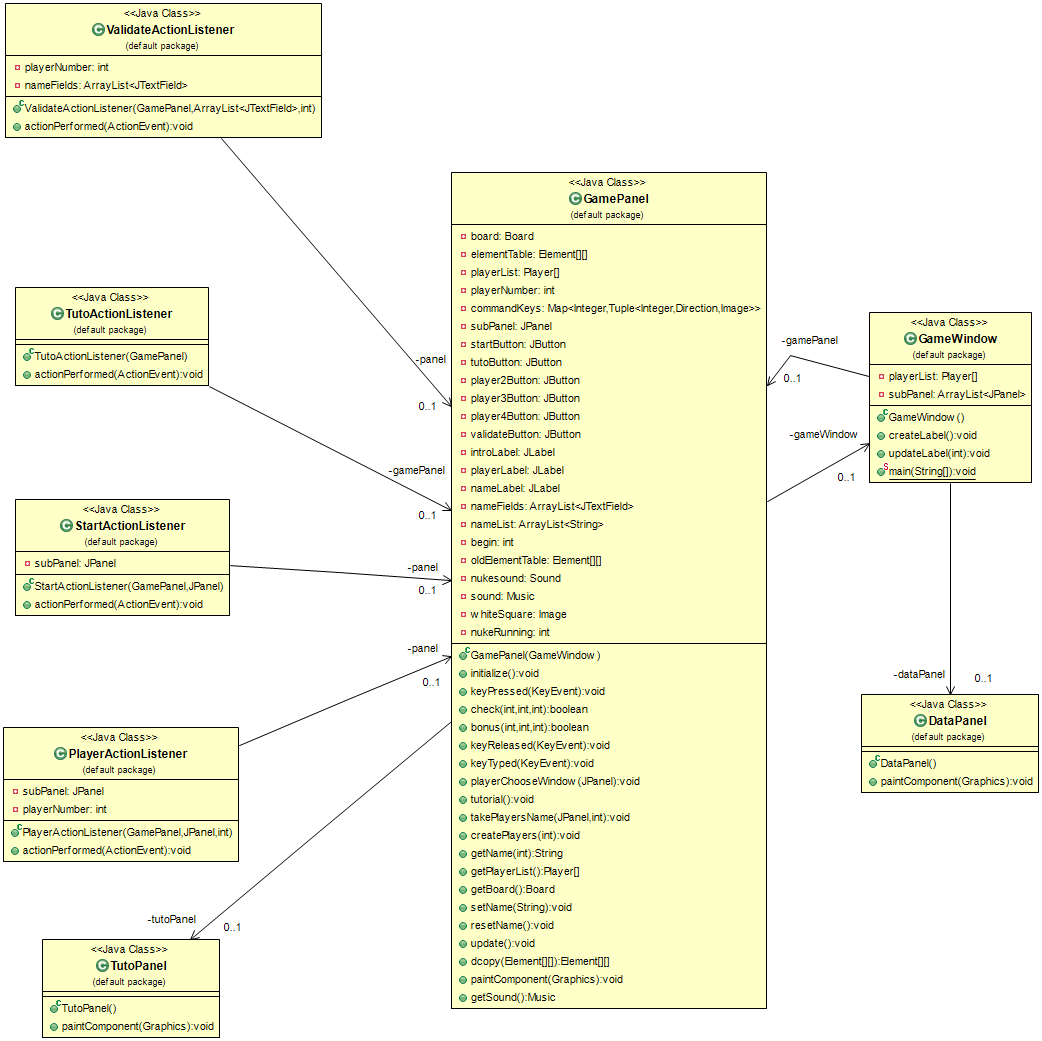
\includegraphics[scale=0.45]{ch1/ViewController}
            \caption {Diagramme des classes : ViewController }
        \end{figure}		
            
        
        \subsubsection{Model}
        Notre \textit{model} se compose d'une interface :
        \begin{enumerate}
            \item \texttt{I Explosion}
        \end{enumerate}
	    et de quatorze classes dont une classe abstraite \texttt{Element}. Les implémentations d'interfaces sont représentées par une $\rightarrow$, 
	    les classes filles par une un <<->> et l'implémentation d'interface entre
        une classe concrète et une interface par $\twoheadrightarrow$\ \footnote{Pour 
        plus de clarté, consultez la \autoref{fig:DiagModel}} :
	    \begin{multicols}{2}
        \begin{itemize}

            \item \texttt{Element}
            \begin{itemize}
            \item[$\rightarrow$] \texttt{Explosion}
				\begin{itemize}
				\item[$\twoheadrightarrow$] \texttt{NonExplosion}
				\item[$\twoheadrightarrow$] \texttt{PlayerExplosion}
				\item[$\twoheadrightarrow$]	 \texttt{BombExplosion}
				\item[$\twoheadrightarrow$]	 \texttt{BlockExplosion}
				\item[$\twoheadrightarrow$]	 \texttt{DeleteExplosion}			
							
				\end{itemize}				            
            
            
	        \item \texttt{Player}
	        \begin{itemize}
			\item[ ]
	        \end{itemize}
            \item \texttt{Bomb}
            \item \texttt{Block}
            \item \texttt{Bedrock}
            \item \texttt{Bonus}
            \item \texttt{Fire}
            \end{itemize}
            \item \texttt{Board}
        
        \end{itemize}
        \end{multicols}
        
        La classe avec laquelle notre contrôleur communique est la classe 
        \texttt{Board}. La classe board crée une matrice remplie d'éléments 
        de type \texttt{Element} : joueurs, différents blocs, bombes, etc. 
        Lorsque l'utilisateur demande d'effectuer un déplacement, celui-ci 
        est renseigné à cette classe via le contr\^oleur pour finalement 
        modifier les attributs de positions du joueur. La matrice remise à 
        jour, un message sera envoyé à la vue afin de remettre à jour l'
        interface graphique.\\
        
        Les différents composants de notre classe \texttt{Board} sont principalement 
        de type \texttt{Element}. La classe \texttt{Element} possède six 
        classes filles : \texttt{Player, Bomb, Block, Bedrock, Bonus et Fire}.
        Le 
        nom des classes est assez explicite si ce n'est pour les deux classes 
        chargées de la gestion des blocs :
        \begin{enumerate}
        \item \texttt{Block} : une case pouvant \^etre détruite suite à l'explosion d'une bombe.
        \item \texttt{Bedrock} : une case ne pouvant \^etre détruite (ainsi 
        qu'une petite référence à \textit{Minecraft}).
        \end{enumerate}
        
        Afin de gérer les explosions de façon la plus efficace que possible, 
        la méthode \textit{explose()} a été définie au sein de la classe 
        \texttt{Element}. Or, cette méthode n'a pas le même comportement pour
        un objet de la classe \texttt{Bedrock} que pour un de la classe \texttt{Bomb,} 
        mais a le m\^eme pour un objet de la classe \texttt{Bonus} (à quelques différences près). 
        Afin que cette méthode puisse être utilisée de façon polymorphe et pour
        éviter les doublons de code, l'interface \texttt{Explosion} implémentée 
        à \texttt{Element} permet de définir un comportement adapté à l'objet
        concerné. Il nous suffira, pour gérer les explosions, d'appliquer une même méthode \textit{applyExplose()} à n’importe quel élément et celui-ci explosera de la manière définie dans la classe correspondante.\\
       
        \begin{center}
        \centering
		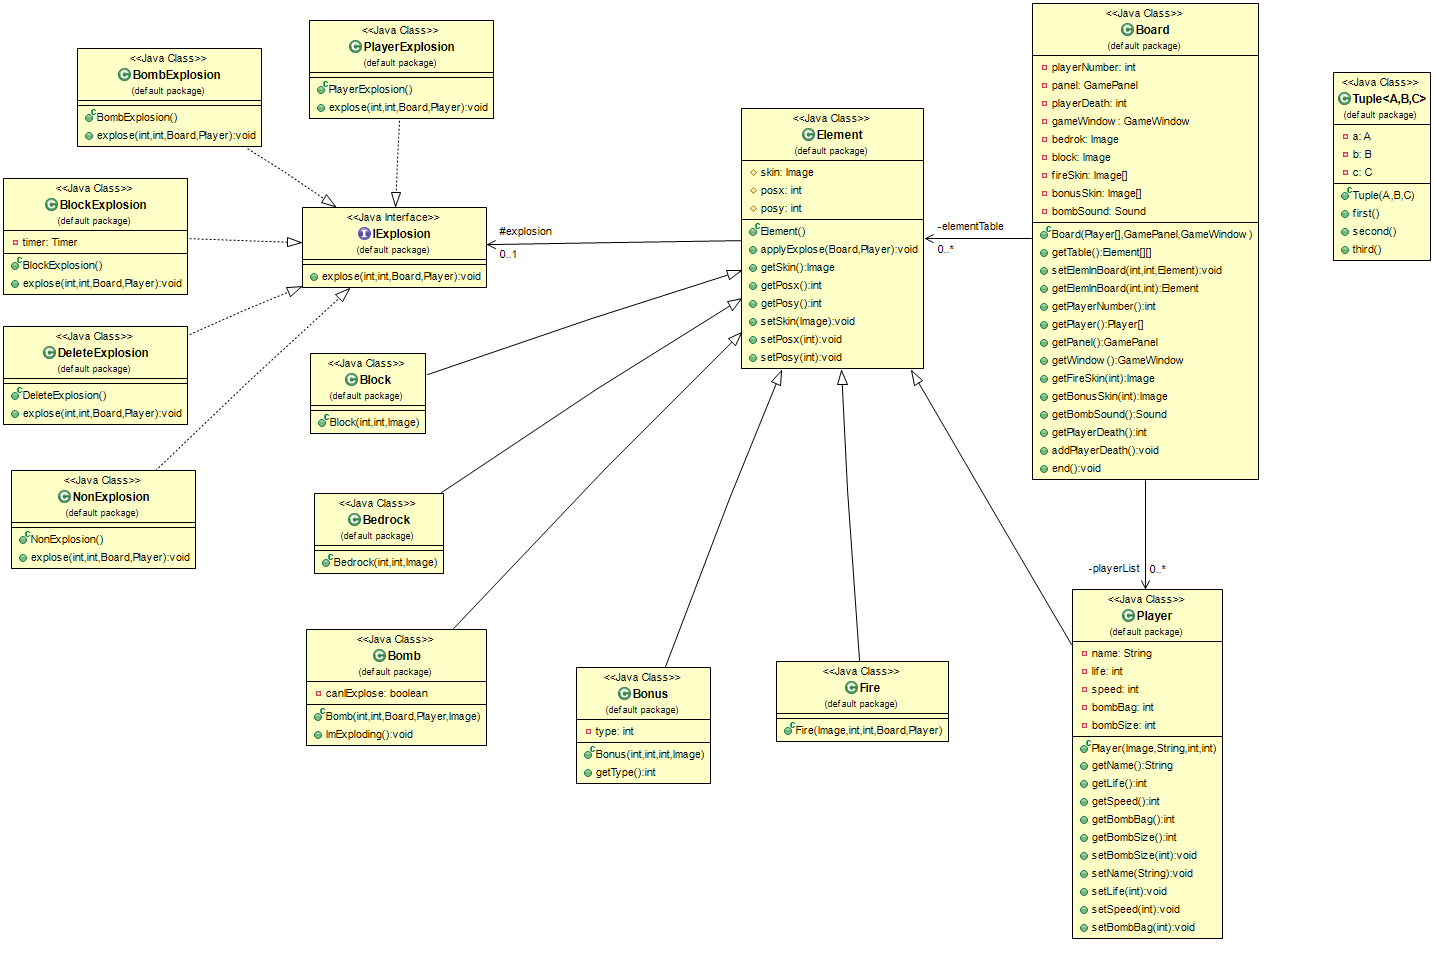
\includegraphics[scale=0.44]{ch1/newModel}
 	 	\captionof{figure}{Diagramme les classes : Model}
 	 	\label{fig:DiagModel}
        \end{center}
        
        
        
        
        
        
        
        
        
        
        
        
        
        
        
        
        
        
        
        
        
        
        
        
        
        
        
        
        
        
		
	

